% !TeX root=_main_.tex
% chapter3

\chapter{کارهای مرتبط}\label{related_work}
\thispagestyle{empty}
\epigraph{
	«یک شب تاریک و طـوفانی بود. پاییز 1994، در آپارتمان خود در مادیـسون نشسته بودم. آن شب من از طریق خط تلفن به سیستم‌های یونیکس دانشگاه متصل شدم. با بارش سنگین باران اختلال زیادی روی خط اتصالی بود که در اجرای فرمان‌های ارسالی من دخالت می‌کرد. رقابتی بین سرعت نوشتن یک فرمان قبل از آنکه اختلال آن را خراب کند وجود داشت. چیزی که مرا شگفت زده می‌کرد این حقیقت بود که اختلال سبب ایجاد خرابی و سقوط برنامه‌ها می‌شد و شگفت‌آورتر برنامه‌هایی بود که سقوط می‌کرد: ابزارهای رایج یونـیکس!»
}
{$ \maltese $ {\large بارتون میلر، مبدع آزمون فازی}}

\noindent
کارهای بسیاری برای بهبود آزمون فازی اولیه که داده‌های آزمون را به‌صورت تصادفی تولید می‌کرد \cite{Miller:1990:ESR:96267.96279}، انجام شده است. فازرهای \gls{GenerationBased} در برنامه‌های با ساختار ورودی پیچیده پوشش کد بیشتری نسبت به فازرهای \gls{MutationBased} فراهم می‌کنند\cite{Miller2007}، اما کاملاً خودکار نیستند \cite{Godefroid:2017:LML:3155562.3155573}. در مقابل فازرهای \gls{MutationBased} سعی کرده‌اند تا با استفاده از الگوریتم ‌های تکاملی مثل ژنتیک داده‌ آزمون‌های بهتری را برای جابه‌جایی انتخاب کنند. \lr{AFL} \cite{Zalewsky2013} نمونه‌ای موفق از فازرهای \gls{MutationBased} است. در سال 2017، فنون یادگیری ماشینی به هر دودسته از فازرهای بالا اعمال شده‌اند. در فازرهای \gls{GenerationBased}، برای یادگیری خودکار گرامر فایل \cite{Godefroid:2017:LML:3155562.3155573} و در فازرهای \gls{MutationBased} برای پیش‌بینی بهترین مکان جابه‌جایی \cite{DBLP:journals/corr/abs-1711-04596}. هریک از این کارها نواقص و محدودیت‌هایی دارند. در این فصل به معرفی، نقد و بررسی این کارها می‌پردازیم.



\section{فازر AFL}
\lr{AFL} \cite{Zalewsky2013}
 یک فازر قالب فایلِ جعبه خاکستری، با تولید داده آزمون مبتنی بر جابه‌جایی، دارای بازخورد، متن‌باز و رایگان است که توسط 
 \lr{Michal Zalewski}\LTRfootnote{\href{http://lcamtuf.coredump.cx/}{http://lcamtuf.coredump.cx/}}
  توسعه داده شده است. این فازر روی سیستم عامل‌های خانواده یونیکس قابل اجرا است. راه‌اندازی آن ساده بوده و واسط کاربری خوبی برای دنبال کردن جزئیات آماری فرایند آزمون فازی و خطاهای کشف شده دارد. در ‏شکل \ref{ch3_afl_gui.png} یک نمونه از اجرای این فازر را در عمل نشان داده‌ایم.
  
  
 به‌طور پیش‌فرض \lr{AFL} برای سنجش پوشش کد، به کد منبع \gls{SUT}  نیاز دارد. برنامه‌های نوشته شده به زبان‌های 
 \lr{C}،
 \lr{C++} و
 \lr{Objective-C}
 در آزمون فازی جعبه سفید با \lr{AFL} قابل استفاده هستند. همچنین نسخه‌هایی از \lr{AFL} برای برنامه‌های نوشته شده به زبان‌های
 	 \lr{Go} و \lr{Python}
 	  توسط دیگران انتشار یافته است. \lr{AFL} در آزمون فازی جعبه سیاه، برای ابزارگذاری و اخذ اطلاعات زمان اجرا، از ابزار
 	   \lr{QEMU} \cite{QEMU2018}
 	   استفاده می‌کند. این فازر به‌حدی موفق بوده‌ که پژوهش‌های زیادی برای بهبود جنبه‌های مختلف آن انجام شده است. اما چنان‌چه خواهیم دید روی قالب فایل‌هایی با ساختار پیچیده نمی‌تواند به پوشش خوبی دست پیدا کند \cite{DBLP:journals/corr/abs-1711-04596}.
 	   
 	   
 \begin{figure}[H]%[tbh!]%[ht]%[t!]
 	   	\centering
 	   	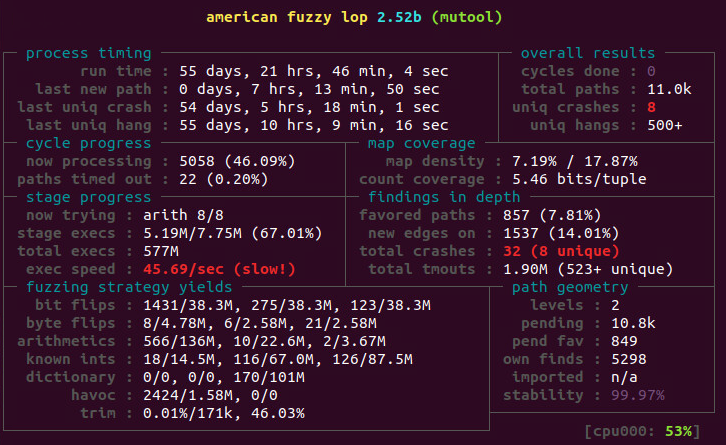
\includegraphics[width=\textwidth, clip=true,  trim= 0 0 0 0]{chapter3/ch3_afl_gui.png}
 	   	\caption[محیط زمان اجرای AFL]
 	   	{
 	اجرای \lr{AFL} بر روی ابزار \lr{mutool}  از نرم‌افزار 
 	\lr{MuPDF} \cite{MuPDF2018}. این تصویر جزئیات اجرا بعد از گذشت 55 روز از آغاز فرایند آزمون فازی را نشان می‌دهد. آزمون تا زمانی که کاربر $ctrl+z$ را فشار ندهد، اجرا می‌شود.
 	   	}
 	   	\label{ch3_afl_gui.png}
 	   	%\ref{ch3_afl_gui.png}
\end{figure}
 	      
 	   
 	   

\subsection{معماری AFL}
‏شکل \ref{ch3_afl_fuzz.png} 
\glspl{Component}ی 
اصلی فازر \lr{AFL}  و ترتیب استفاده از آنها در هنگام آزمون فازی را نشان می‌دهد. در این معماری چهار \gls{Component} مشاهده می‌شود: 

 \begin{figure}%[tbh!]%[ht]%[t!]
	\centering
	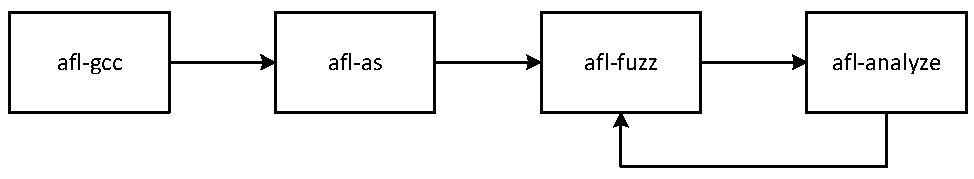
\includegraphics[width=0.95\textwidth, clip=true,  trim= 0 0 0 0]{chapter3/ch3_afl_fuzz.pdf}
	\caption[مؤلفه‌های فازر \lr{AFL} و ارتباط آنها]
{
	مؤلفه‌های فازر \lr{AFL} و ارتباط آنها با یکدیگر
	\cite{Zalewsky2013}.
}
\label{ch3_afl_fuzz.png}
%\ref{ch3_afl_fuzz.png}
\end{figure}



\begin{itemize}
	\item {
	\textbf{\lr{afl-gcc}.}
	یک جایگزین برای \lr{gcc}  یا \lr{clang}  استاندارد است که برای کامپایل کد منبع \lr{SUT}  استفاده می‌شود و خروجی آن به \lr{afl-as}  ارسال می‌شود. در رویکرد جعبه سفید استفاده مرحله اول کامپایل \lr{SUT} با
	 \lr{afl-gcc}
	  است.

}
\item {
	\textbf{\lr{afl-as}.}
	کد کامپایل شده با \lr{afl-gcc} را با تزریق کدهای اسمبلی ابزارگذاری می‌کند. ابزارگذاری به نحوی است که پوشش انشعاب  یا پرش را ضبط می‌کند. خروجی \lr{afl-as}  فایل دودویی قابل اجرای \lr{SUT}  است که سپس توسط
	 \lr{afl-fuzz}
	  استفاده می‌شود.
}
\item {
\textbf{\lr{afl-fuzz}.}
همانطور که انتظار می‌رود، هسته اصلی فازر است که عملیات فاز ورودی را انجام می‌دهد. این ابزار فایل دودویی و داده آزمون ورودی را دریافت و با توجه به اطلاعات دریافتی از \lr{afl-analyze} فرایند آزمون را ادامه می‌دهد. این مؤلفه برای آزمون فازی جعبه سیاه، مستقیماً به‌کار می‌رود. \lr{afl-fuzz} همچنین مسئول چاپ واسط کاربری روی ترمینال است.
}

\item {
\textbf{\lr{afl-analyze}.}
 اثر ورودی اجرا شده بر پوشش کد را بررسی می‌کند و اطلاعات مربوط به پوشش کد را به عنوان بازخوردی به \lr{afl-fuzz} می‌دهد تا برای جابه‌جایی‌های بهتر در ادامه استفاده کند.
}

\end{itemize}
 
حلقه بازخوردی که در ‏شکل \ref{ch3_afl_fuzz.png} وجود دارد نشان دهنده تکاملی بودن فرایند آزمون فازی در \lr{AFL} است. \lr{AFL} در هسته خود از الگوریتم ژنتیک استفاده می‌کند. یک فایل ورودی جهش یافته، مفید و مورد توجه است اگر قسمت‌های جدیدی از کد دودویی را اجرا کرده باشد یا تعداد اجرای کدهای قبلی مشاهده شده را افزایش داده باشد. این ویژگی با عنوان \lr{Input Gain} شناخته می‌شود \cite{DBLP:journals/corr/abs-1711-04596}. \lr{AFL}، سپس این داده آزمون را به انتهای صف داده‌های آزمون، اضافه می‌کند. به این ترتیب حاصل فرایند آزمون فازی در \lr{AFL}، علاوه بر اجرای \gls{SUT} و اندازه‌گیری پوشش کد، یک مجموعه داده آزمون جهش یافته با ویژگی‌های متمایز است. 


برای مقایسه نحوه عملکرد \lr{AFL} و یک فازر تصادفی، جزئیات الگوریتم‌های این دو فازر را مرور می‌کنیم. الگوریتم \ref{alg:random_fuzz}، فرایند فاز ورودی در یک فازر تصادفی و الگوریتم \ref{alg:afl_fuzz} همین فرایند را در \lr{AFL} نشان می‌دهد. تابع $ Mutate $ یک بایت از ورودی را به‌صورت درجا، با استفاده از فنونی مثل وارون‌کردن بیت، وارون‌کردن بایت، چرخش بیت‌ یا عملیات ریاضی و منطقی، جابه‌جا می‌‌کند. تابع $ Execute $ برنامه را با ورودی جابه‌جا شده اجرا و خرابی‌های احتمالی را گزارش می‌دهد. خطوط سایه زده شده در دو الگوریتم (خطوط 10، 14 و 15) قسمت‌های متفاوت را نشان می‌دهد \cite{DBLP:journals/corr/abs-1711-04596}. 


  
 %\begin{figure*}[t]
 %\centering
 %\removelatexerror
 %\begin{minipage}[t]{9cm}
 %	\vspace{0pt}
 \begin{algorithm}[ht]%[H]%
 	\onehalfspacing
 	\caption[\lr{Basic-Random Fuzzing}]{\lr{Basic-Random Fuzzing} \cite{DBLP:journals/corr/abs-1711-04596}} \label{alg:random_fuzz}
 	
 	\begin{latin}
 		\DontPrintSemicolon
 		\setcounter{AlgoLine}{0}
 		\LinesNumbered
 		
 		%\TitleOfAlgo{Simple Random Fuzzing}
 		
 		\SetKwFunction{RandInt}{RandInt}
 		\SetKwFunction{len}{len}
 		\SetKwFunction{mutate}{mutate}
 		\SetKwFunction{Execute}{Execute}
 		
 		\SetKwInput{KwData}{Input}
 		\SetKwInput{KwResult}{Output}
 		
 		\KwData{$Seeds$, Target program $P$}
 		\KwResult{$MaliciousInputs$}
 		
 		\For{$Seed$ $\in$ $Seeds$}{
 			
 			\For{$iterations \gets 0$ \KwTo $limit$ }{
 				
 				$input \gets Seed$
 				
 				$length \gets$ \len{$Seed$}
 				
 				$mutations \gets$ \RandInt{$length$}
 				
 				\For{$mut \gets 0$ \KwTo $mutations$}{
 					
 					$byte \gets$ \RandInt{$length$}
 					
 					\mutate{$input$, $byte$}
 				}
 				
 				\HiLi $result \gets$ \Execute{$P$, $input$}
 				
 				\If {$result$ is crash}{
 					
 					Append $input$ to $MaliciousInputs$
 				}
 				
 				\HiLi \;
 				
 				\HiLi \;
 				
 				\;
 			}
 			
 		}
 		
 	\end{latin}
 	
 	
 \end{algorithm} 
 %\end{minipage}%
 
 
 %\begin{minipage}[t]{9cm}
 %	\vspace{0pt}
 \begin{algorithm}[ht]%[H]
 	\onehalfspacing
 	\caption[\lr{AFL Fuzzing}]{\lr{AFL Fuzzing} \cite{DBLP:journals/corr/abs-1711-04596}} \label{alg:afl_fuzz}
 	
 	\begin{latin}
 		\DontPrintSemicolon
 		\setcounter{AlgoLine}{0}
 		\LinesNumbered
 		
 		%\TitleOfAlgo{AFL Fuzzing}
 		
 		\SetKwFunction{RandInt}{RandInt}
 		\SetKwFunction{len}{len}
 		\SetKwFunction{Mutate}{Mutate}
 		\SetKwFunction{Execute}{Execute}
 		\SetKwFunction{HasInputGain}{HasInputGain}
 		
 		\SetKwInput{KwData}{Input}
 		\SetKwInput{KwResult}{Output}
 		
 		\KwData{$Seeds$, Target program $P$}
 		\KwResult{$MaliciousInputs$}
 		\For{$Seed$ $\in$ $Seeds$}
 		{
 			\For{$iterations \gets 0$ \KwTo $limit$ }{
 				$input \gets Seed$
 				
 				$length \gets$ \len{$Seed$}
 				
 				$mutations \gets$ \RandInt{$length$}
 				
 				\For{$mut \gets 0$ \KwTo $mutations$}
 				{
 					$byte \gets$ \RandInt{$length$}
 					
 					\Mutate{$input$, $byte$}
 					
 				}
 				
 				\HiLi $result, cov \gets$ \Execute{$P$, $input$}
 				
 				\If {$result$ is crash}
 				{
 					Append $input$ to $MaliciousInputs$
 				}
 				\HiLi \If {\HasInputGain{cov}}
 				{
 					\HiLi  Append $input$ to $Seeds$
 				}
 				
 			}
 		}
 		
 	\end{latin}
 	
 \end{algorithm} 
 %\end{minipage}%
 %%%%%%%%
 % \end{figure*}


\subsection{مشکلات AFL}
آزمون فازی از لحاظ محاسباتی سنگین است. یعنی حتی یک \lr{Input Gain} کوچک نیاز نیازمند هزارها تا میلیون‌ها جابه‌جایی است \cite{DBLP:journals/corr/abs-1711-04596}. از طرفی همه جابه‌جایی‌های یکسان نیستند. \lr{AFL} با بهره‌گیری از بازخورد داده‌های آزمون بهتری را انتخاب می‌کند، اما همچنان آنها را به صورت تصادفی جهش می‌دهد یا جابه‌جا می‌کند. در نتیجه تعداد زیادی داده آزمون تکراری تولید می‌شود که لزوما تأثیری بر بهبود آزمون ندارند. از طرفی در ساختارهای پیچیده، تغییر برخی قسمت‌ها سبب می‌شود تا داده آزمون ورودی نامعتبر شود و سریعاً توسط تجزیه‌گر مردود اعلام گردد. در نتیجه تعداد زیادی داده آزمون هدر رفته خواهیم داشت. \lr{AFL}\gls{Augmented}
\cite{DBLP:journals/corr/abs-1711-04596}
مسئله انتخاب تصادفی مکان‌های جابه‌جایی را مورد مطالعه و راه‌کارهایی برای هوشمندسازی آن ارائه داده است (بخش \ref{sec:augmented-afl}). 


محدودیت دیگر \lr{AFL} \gls{Portability} پایین آن است. \lr{AFL} به‌خاطر استفاده از فراخوانی‌های سیستمی سیستم‌ عامل \lr{Linux} تنها در توزیع‌های آن قابل استفاده است. نسخه‌‌ای از \lr{AFL}، تحت عنوان
 \lr{WinAFL}\LTRfootnote{\href{https://github.com/ivanfratric/winafl}{https://github.com/ivanfratric/winafl}}
برای سیستم عامل ویندوز توسعه داده شده است که البته سرعت پایین و سربار بالایی دارد. \lr{WinAFL} برای افزایش سرعت پیشنهاد می‌کند که تنها یک تابع از برنامه که هدف اصلی آزمون فازی است، ابزارگذاری شود.

به‌دلیل مشکلاتی که اشاره شد، اجرای \lr{AFL} و هرگونه فازر مشابه آن، روی نرم‌افزارهایی مثل \gls{PDF}خوان‌ها که ساختار ورودی آنها پیچیده است به پوشش کد به‌مراتب کمتری دست می‌یابد که حتی با افزایش زمان آزمون نیز نتایج بهبود چندانی نمی‌کند. در این پایان‌نامه یک روش ترکیبی برای تولید داده آزمون ارائه می‌دهیم که پوشش کد بهتری نسبت به فازرهای مبتنی بر جابه‌جایی محض برای ساختارهای پیچیده فراهم کرده و در عین حال ویژگی‌های مثبت جابه‌جایی در فایل‌های دودویی را نیز به‌کار می‌بنند.



\section{فازر \lr{AFL}افزوده}\label{sec:augmented-afl}
 \lr{AFL}افزوده \cite{DBLP:journals/corr/abs-1711-04596} 
تلاش می‌کند با استفاده از فنون یادگیری ماشینی مکان‌های مناسبی را برای جابه‌جایی بایت‌ها پیدا کند. چارچوب ارائه شده در این کار شامل فازر \lr{AFL} و یک  مدل است که مکان‌های مفید برای جابه‌جایی را مشخص می‌کند. در طول اجرا فازر ابتدا مدل را برای اخذ آدرس مکان‌های جهش پرس‌وجو می‌کند و جابه‌جایی‌های فازر را روی مکان‌های بازگردانیده شده متمرکز می‌کند.

برای آموزش مدل فایل ورودی از مجموعه دانه اولیه، فایل جهش یافته و میزان پوشش کد هر دو فایل پس از اجرا توسط \gls{SUT} مورد نیاز است. در فرایند آموزش اگر پوشش کد فایل جهش یافته و فایل والد یکسان باشد (یعنی میزان \lr{Input Gain} صفر باشد)، مکان‌های جابه‌جا شده مکان‌های امیدبخشی نخواهند بود و چنان‌چه پوشش کد فایل جابه‌جا شده افزایش داشته باشد (یعنی میزان \lr{Input Gain} بزرگ‌تر از صفر باشد)، آنگاه جابه‌جایی‌ها امیدبخش محسوب می‌شوند. با تعریف یک تابع خطا که بسته به مقدار \lr{Input Gain} امتـیاز‌هایی به هریک از دو حالت بالا نسبت می‌دهد، مدل در حالت بانظارت آموزش می‌بیند. ورودی مکان‌های جهش در فایل و خروجی میزان امتیاز کسب شده بر اثر هریک از این‌ مکان‌ها است. صورت‌بندی ریاضی مطالب عنوان شده، به‌طور مفصل در \cite{DBLP:journals/corr/abs-1711-04596} ذکر شده است.

 یک ویژگی مثبت این مقاله آموزش و استفاده از چندین مدل متنوع یادگیری ژرف و نیز آزمون چندین برنامه هدف در انجام آزمایش‌ها است که سبب می‌شود تأثیر مدل‌های مختلف را بتوان با یکدیگر مقایسه کرد. برای ایجاد مجموعه آموزش، فازر \lr{AFL} با تعداد 180 دانه اولیه برای هر \gls{SUT} به مدت 24 ساعت اجرا گردیده و اطلاعات لازم ضبط شده‌اند.
 
 الگوریتم \ref{alg:augmented-afl_fuzz}، فرایند فاز ورودی و انجام آزمون فازی در \lr{AFL}افزوده را نشان ‌می‌دهد. خطوط سایه زده شده (خطوط 2، 11، 12 و 13) قسمت‌های اضافه شده به الگوریتم اصلی \lr{AFL}  هستند. 
 چون جابه‌حایی‌های \lr{AFL} در حالت عادی به‌صورت تصادفی است (خطوط 7 و 8 در الگوریتم \ref{alg:afl_fuzz} و خطوط 8 و 9 در الگوریتم \ref{alg:augmented-afl_fuzz})،
  تغییر انجام شده در \lr{AFL}افزوده بدین صورت است که ابتدا مکان‌های مناسب جابه‌جایی برای یک ورودی را توسط مدل پیش‌بینی می‌کند، سپس اجازه می‌دهد تا \lr{AFL}  ورودی را جابه‌جا کند. 
  حال چنان‌چه مجموع شباهت جابه‌جایی‌های \lr{AFL} با جابه‌جایی‌های گزارش شده که مطلوب مدل است، کمتر از یک حد آستانه $ \alpha$  باشد (خط 12 الگوریتم \ref{alg:augmented-afl_fuzz})؛
  این داده آزمون تولیدی برای اجرا ارسال نمی‌گردد. محاسبه شباهت دو رشته بیتی نیز با استفاده از ترکیب عطفی آنها (خط 12 الگوریتم \ref{alg:augmented-afl_fuzz}) به‌‌راحتی امکان‌پذیر است. چنان‌چه دو رشته مشابه نباشند مجموع بیت‌های ترکیب عطفی آنها کمتر از مجموع بیت‌های هریک از  آنها خواهد بود و بالعکس.
  
 
 \begin{algorithm}%[ht]%[H]
	\onehalfspacing
	\caption[\lr{Augmented-AFL Fuzzing}]{\lr{Augmented-AFL Fuzzing}  \cite{DBLP:journals/corr/abs-1711-04596}} \label{alg:augmented-afl_fuzz}
	
	\begin{latin}
		\DontPrintSemicolon
		\setcounter{AlgoLine}{0}
		\LinesNumbered
		
		%\TitleOfAlgo{Augmented-AFL Fuzzing}
		
		\SetKwFunction{RandInt}{RandInt}
		\SetKwFunction{len}{len}
		\SetKwFunction{Mutate}{Mutate}
		\SetKwFunction{Execute}{Execute}
		\SetKwFunction{HasInputGain}{HasInputGain}
		\SetKwFunction{QueryModel}{QueryModel}
		\SetKwFunction{Sum}{Sum}
		
		\SetKwInput{KwData}{Input}
		\SetKwInput{KwResult}{Output}
		
		\KwData{$Seeds$, Target program $P$}
		\KwResult{$MaliciousInputs$}
		
		\For{$Seed$ $\in$ $Seeds$}{
			
			\HiLi $bytemask \gets$ \QueryModel{$Seed$}
			
			\For{$iterations \gets 0$ \KwTo $limit$ }{
				
				$input \gets Seed$
				
				$length \gets$ \len{$Seed$}
				
				$mutations \gets$ \RandInt{$length$}
				
				\For{$mut \gets 0$ \KwTo $mutations$}
				{
					$byte \gets$ \RandInt{$length$}
					
					\Mutate{$input$, $byte$}
					
				}
				
				\HiLi $\mathit{diff}$ $\gets input \oplus Seed$
				
				\HiLi \If{$\sum \mathit{diff}$ $\land$ $bytemask$ < $\alpha$}
				{
					\HiLi   \textbf{Continue}
				}
				
				$result, codecov \gets$ \Execute{$P$, $input$}
				
				\If {$result$ is crash}
				{
					Append $input$ to $MaliciousInputs$
				}
				
				\If {\HasInputGain{codecov}}
				{
					Append $input$ to $Seeds$
				}
			}
		}
	
	\end{latin}%
	
\end{algorithm}%

%%%

\subsection{مشکلات \lr{AFL}افزوده}\label{sec:augmented_afl_problems}

الگوریتم \lr{AFL}افزوده روی چندین قالب فایل و چندین برنامه محتلف، مورد آزمایش قرار گرفته است؛ از جمله قالب‌های فایل
	 \lr{PNG}، \lr{XML} و \lr{PDF}. کمترین بهبود گزارش شده بازهم مربوط به قالب فایل \lr{PDF} و نرم‌افزار \lr{MuPDF} است. علت آن هم ساختار پیچیده و هم حجم بالای فایل‌های \lr{PDF} است. 
	 میزان درصد پوشش کد گزارش شده برای نرم‌افزار \lr{MuPDF} توسط \lr{AFL} اصلی 
	 $11.63$
	 و توسط \lr{AFL}افزوده در بهترین مدل $11.80$ بوده که افزایش ناچیز $0.17$ درصدی را نشان می‌دهد. در بخش نتایج این مقاله همچنین هیچ ارزیابی روی دقت مدل‌های مختلف آموزش داده شده انجام نشده و به یک نتیجه‌گیری کلی بسنده شده است.
	 
	 یک تأکید مهم که در مستندات \lr{AFL} به آن اشاره شده است کوچک نگاه‌ داشتن فایل‌های مجموعه دانه اولیه است (توصیه شده است که از فایل‌هایی با حجم زیر 1 کیلوبایت استفاده شود)؛ زیرا، در صورتی که از فایل‌های با حجم بالایی استفاده شود سرعت فازر به‌شدت کاهش می‌یابد. در واقع جابه‌جایی‌های بسیاری بایستی روی یک دانه اعمال گردد تا یک داده آزمون جدید ایجاد شود. این در حالی است که برخی ساختارها مثل \lr{PDF} ذاتاً حجم بالایی دارند. مثلاً یک فایل \lr{PDF} تنها حاوی عبارت 
	 \lr{Hello Wrold}
	 حجمی در حدود 1 کیلوبایت دارد.
	 برای این ساختارها، تولید یک فایل جدید از ابتدا، مثلاً از روی یک مدل، سرعت تولید داده آزمون را افزایش می‌دهد. استفاده از یک روش ترکیبی یعنی ثابت نگه داشتن بخش‌هایی از فایل و تولید بخش‌های دارای اهمیت در ساختار یک فایل سرعت تولید داده را حتی بیشتر از تولید یک فایل از ابتدا هم افزایش می‌دهد. روش ارائه شده در این پایان‌نامه یک روش ترکیبی است.
	 

	 
%%%%%%%%%%%%%%%%%%%%%%%
%%% Learn and Fuzz  %%%
%%%%%%%%%%%%%%%%%%%%%%%

\section{یادگیری و فاز}
    
مقاله \gls{LearnAndFuzz} \cite{Godefroid:2017:LML:3155562.3155573} روشی برای تولید داده آزمون جهت استفاده در آزمون فازی بر مبنای  \gls{RNN} و مدل \gls{EncoderDecoder} \cite{DBLP:journals/corr/ChoMGBSB14,NIPS2014_5346} ارائه کرده است. در این مقاله ساختار فایل  \gls{PDF} و مرورگر وب
 \lr{Edge}\footnote{مرورگر جدید شرکت مایکروسافت که همراه با سیستم عامل ویندوز 10 معرفی شد.}
  شرکت مایکروسافت، برای آزمون انتخاب شده‌اند. ایده اصلی یادگیری یک مدل مولد زبان روی مجموعه‌ای از ویژگی‌های اشیای \gls{PDF} با داشتن مجموعه‌ای از نمونه‌های اولیه است. ساختار قالب فایل \gls{PDF} و اشیای داده‌ای آن، در پیوست آ توضیح داده شده است.

مدل \gls{EncoderDecoder} \cite{DBLP:journals/corr/ChoMGBSB14,NIPS2014_5346} از دو \gls{RNN} تشکیل شده است. یک شبکه کدگذار که یک توالی ورودی با بُعد متغیر را به یک نمایش بعد ثابت تبدیل می‌کند (بردار زمینه) و یک شبکه کدگشا که یک توالی ورودی بُعد ثابت را می‌گیرد و به یک توالی ورودی با بعد متغیر تولید می‌کند. شبکه کدگشا توالی‌‌های خروجی را با استفاده از کاراکتر خروجی پیش‌بینی شده که در مرحله‌زمانی $ t $ به عنوان کاراکتر ورودی برای مرحله‌زمانی  $ t+1 $ تولید شده است، تولید می‌کند. یک بازنمایی از معماری این مدل در ‏شکل \ref{ch3_encoder_decoder_model_crop.png} نشان داده شده است. این مدل نخستین بار در وظیفه ترجمه ماشینی استفاده شده است \cite{DBLP:journals/corr/ChoMGBSB14}. با توصیف بیان شده، این معماری امکان یادگیری توزیع شرطی 
$ p(<y^{(1)}, y^{(2)}, y^{(3)}, ..., y^{(n)}>| <x^{(1)}, x^{(2)}, x^{(3)}, ..., x^{(n)}>) $ 
را فراهم می‌کند.

\begin{figure}%[tbh!]%[ht]%[t!]
	\centering
	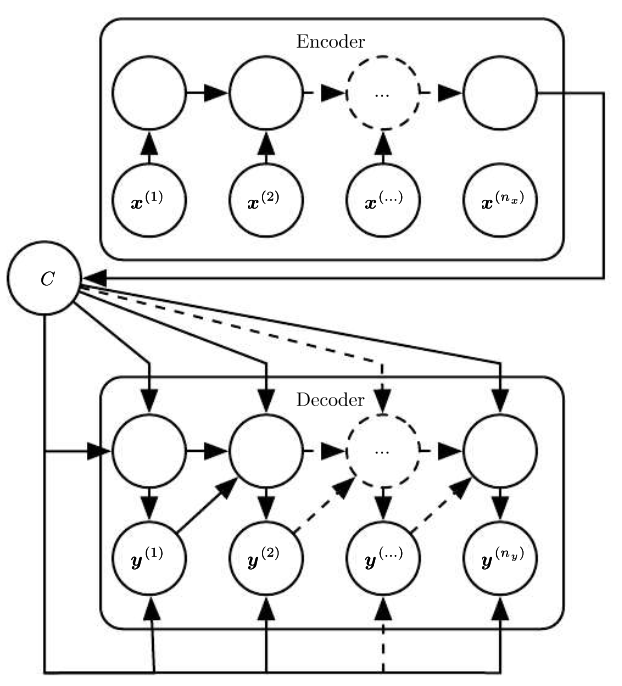
\includegraphics[width=0.7\textwidth, clip=true,  trim= 0 0 0 0]{chapter3/ch3_encoder_decoder_model_crop.png}
	%\includegraphics[width=\textwidth]{figs/chapter1/ch1_fuzz_testing_flowchart2.png}
	\caption[مدل \gls*{EncoderDecoder}]
	{
		مثالی از معماری مدل کدگذار-کدگشا، متشکل از دو \gls{RNN} و بردار زمینه \lr{C}. این مدل برای یادگـیری تولید توالی خروجی 
		$ <y^{(1)}, y^{(2)}, y^{(3)}, ..., y^{(n_y)}> $ 
		 از روی بردار زمینه، که نماینده توالی ورودی 
		$ <x^{(1)}, x^{(2)}, x^{(3)}, ..., x^{(n_x)}> $ 
		  است، به‌کار می‌رود \cite{Goodfellow-et-al-2016}.
	}
	\label{ch3_encoder_decoder_model_crop.png}
	%\ref{ch3_encoder_decoder_model_crop.png}
\end{figure}

\subsection{آموزش مدل کدگذار-کدگشا}
مدل کدگذار-کدگشا در روش یادگیری و فاز، با استفاده از تکه‌ اشیای \gls{PDF} که هر یک به‌صورت توالی‌ای از کاراکترها در نظر گرفته شده است، آموزش می‌بیند. برای آموزش، ابتدا همه فایل‌های حاوی اشیای \gls{PDF} به‌شکل یک توالی از کاراکترها به یکدیگر الحاق  می‌شوند که منجربه ایجاد یک توالی بزرگ از کاراکترها به‌صورت 
$ \hat{s} = <s^{(1)}, s^{(2)}, s^{(3)}, ..., s^{(n)}> $
 خواهد شد. سپس توالی $ \hat{s} $ به چند زیر توالی آموزشی با طول ثابت $ d $ شکسته می‌شود به نحوی که $ i $امین نمونه آموزشی عبارت است از: 
 $ t_i = \hat{s}[i*d: (i+1)*d] $
  که 
  $ s[l:u] $
  یک زیرتوالی از $ s $ بین اندیس‌های $ l $ و $ u $ را نشان می‌دهد. در ادامه، توالی خروجی برای هر توالی آموزشی $ t_i $ عبارت است از توالی ورودی که یک واحد به سمت راست شیفت داده شده است؛ یعنی:
  $ o_{t_i} = \hat{s}[i*d+1: (i+1)*d+1] $.
  مدل سپس به‌صورت \gls{EndToEnd} آموزش می‌بیند تا یک مدل مولد روی مجموعه همه توالی‌های ایجاد شده، یادگیری شود. شکل \ref{ch3_learn_and_fuzz_model_crop.pdf} مدل ارائه شده در این مقاله را نشان می‌دهد.

\begin{figure}%[tbh!]%[ht]%[t!]
	\centering
	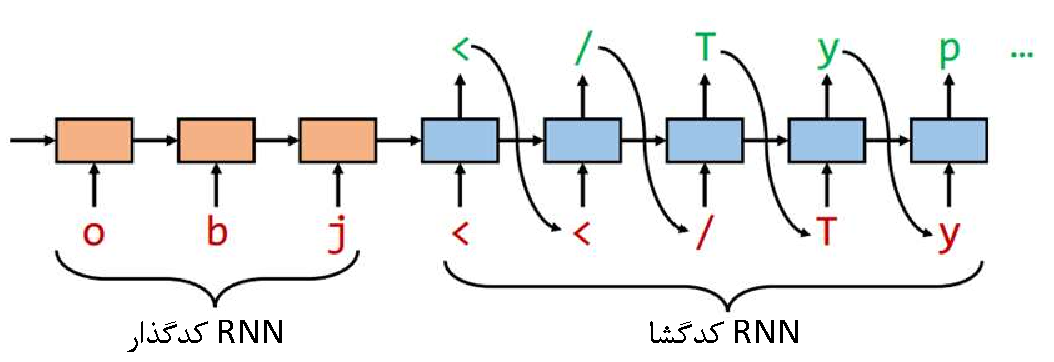
\includegraphics[width=\textwidth, clip=true,  trim= 0 0 0 0]{chapter3/ch3_learn_and_fuzz_model_crop.pdf}
	%\includegraphics[width=\textwidth]{figs/chapter1/ch1_fuzz_testing_flowchart2.png}
	\caption[مدل \gls*{RNN} \gls*{EncoderDecoder} برای تولید اشیای داده‌ای \gls*{PDF}]
	{
		مدل \gls{RNN} \gls{EncoderDecoder} برای تولید اشیای داده‌ای \gls{PDF} \cite{Godefroid:2017:LML:3155562.3155573}.
	}
	\label{ch3_learn_and_fuzz_model_crop.pdf}
	%\ref{ch3_learn_and_fuzz_model_crop.pdf}
\end{figure}


از آنجایی که مدل بحث شده در حالت بدون نظارت آموزش می‌بیند، برچسب‌های تولید شده به‌طور صریح برای مشخص کردن این که مدل یادگرفته شده چه‌قدر خوب عمل می‌کند، آزموده نشدند. به‌جای آن چندین مدل آموزش داده می‌شود که در تعداد دوره‌ها (بخش \ref{feedforwardtraining}) متفاوت هستند. مدل در 10، 20، 30، 40 و 50 دوره آموزش داده شده است. در تنظیمات شبکه ارائه شده در این مقاله، یادگیری روی هر دوره حدود 12 دقیقه طول می‌کشد و بنابراین مدل با 50 عدد حدودا 10 ساعت زمان نیاز دارد تا کامل شود. شبکه به‌صورت \gls{RNN} با 2 لایه مخفی که هر لایه 128 سلول \gls{LSTM} دارد، است.


\subsection{تولید داده‌های جدید}\label{sec:new_data_generation}
از مدل یادگیری شده برای تولید اشیای جدید \gls{PDF} استفاده شده است. راهبردهای مختلفی برای تولید اشیا، بسته به راهبرد نمونه‌برداری که برای نمونه‌برداری از توزیع یادگیری شده به‌کار می‌رود، وجود دارند. در این مقاله، با یک \gls{Prefix} از توالی \texttt{"obj"} (که آغاز یک شی را مشخص می‌کند) شروع و سپس مدل را پرس‌وجو کرده تا یک توالی از کاراکترهای خروجی تولید گردد، تا زمانی که مدل \texttt{"endobj"} را که مشخص کننده انتهای یک شی است، تولید نماید. سپس این مقاله، سه راهبرد مختلف را برای تولید اشیای جدید از روی مدل، استفاده کرده است \cite{Godefroid:2017:LML:3155562.3155573}:

\begin{itemize}
	\item{
		\textbf{\lr{NoSample}.}
	 در این راهبرد تولید، کاراکتر پیش‌بینی شده با بالاترین احتمال به‌عنوان کاراکتر بعدی انتخاب می‌شود که در واقع انتخابی \gls{Greedy} است. این راهبرد برای تولید اشیای \gls{PDF}ای که \gls{Wellformed} و \gls{Consistent} هستند، کاملاً نتیجه‌بخش است ولی تعداد اشیائی را که می‌توان تولید کرد، محدود می‌کند. با دادن یک پیشوند مثل  \texttt{"obj"}  بهترین توالی از کاراکترهای بعدی به‌صورت یکتا مشخص می‌شود و بنابراین این راهبرد همان شی را نتیجه می‌دهد. این محدودیت مغایر با اهداف آزمون فازی بوده و مانع مفید بودن استفاده از آن در آزمون فازی می‌شود. 
}
\item{
	\textbf{\lr{Sample}.}
در این راهبرد تولید، به‌جای انتخاب محتمل‌ترین کاراکتر پیش‌بینی شده، از توزیع یادگرفته شده، برای نمونه‌برداری کاراکتر بعدی در توالی‌ای که پیشوند آن داده شده است، استفاده می‌شود. راهبرد نمونه‌برداری قادر به تولید مجموعه گوناگونی از اشیا با ترکیب الگوهای مختلفی که از اشیای موجود یادگرفته شده است، خواهد بود. به دلیل نمونه‌برداری اشیای تولید شده، تضمینی نیست که آنها به میزان راهبرد قبلی،  \gls{Wellformed} باشند، که این ویژگی از منظر آزمون فازی مفید است.
}

\item{
	\textbf{\lr{SampleSpace}.}
این راهبرد ترکیب دو راهبرد قبلی است. \lr{SampleSpace} توزیع احتمالی برای تولید کاراکتر بعدی را تنها زمانی که پیشوند توالی کنونی، با فضای خالی خاتمه می‌یابد، نمونه‌برداری می‌کند. برای میان \gls{Token}‌ها (یعنی پیشوندهایی که با فضای خالی خاتمه نمی‌یابند)، بهترین کاراکتر را انتخاب می‌کند (راهبرد \lr{NoSample}) است که در مقایسه با راهبرد \lr{Sample}،  ورودی‌های خوش‌شکل‌تری تولید می‌شود. چون نمونه‌برداری در پایان کاراکترهای فضای خالی صورت می‌گیرد؛ نمونه‌های جدید نیز در این راهبرد، ساخته خواهند شد.
}
\end{itemize}

\subsection{اعمال آزمون فازی}

برای فاز داده‌های آزمون تولید شده، مقاله الگوریتم جدیدی تحت عنوان \lr{SampleFuzz} ( الگوریتم \ref{alg:sample_fuzz})، ارائه کرده است. \lr{SampleFuzz} توزیع یادگیری شده
 $ D(x,\theta) $،
احتمال فازینگ یک کاراکتر $ t\_fuzz $ و احتمال آستانه‌ $ p\_t $ که تصمیم می‌گیرد آیا کاراکتر پیش‌بینی شده اصلاح شود یا نه، را به عنوان ورودی می‌پذیرد. سپس برای توالی خروجی $  seq $، الگوریتم $ D(x,\theta) $ را نمونه‌برداری می‌کند تا کاراکتر بعدی یعنی $ c $ و احتمال آن $ p(c)$ را در یک مرحله زمانی مشخص $ t $ به‌دست آورد. اگر احتمال $ p(c)$ از آستانه فراهم شده توسط کاربر ($ p\_t $) بالاتر باشد؛ یعنی، اگر مدل مطمئن باشد که کاراکتر بعدی به احتمال زیاد  $ c $ است، الگوریتم تصمیم می‌گیرد تا یک کاراکتر دیگر $ c' $ که احتمال کمینه $ p(c') $ را دارد، جایگزین $ c $ کند. البته این اصلاح (فاز) تنها در صورتی که عدد تصادفی تولید شده $ p\_fuzz $ از ورودی $ t\_fuzz $  مقدار بیشتری داشته باشد، انجام می‌شود، که بدین ترتیب اجازه می‌دهد تا کاربر بتواند بر روی احتمال (درصد) کاراکترهای فاز شده کنترل داشته ‌باشد.

 
\begin{algorithm}[ht]
	\onehalfspacing
	\caption[\lr{SampleFuzz}]{\lr{SampleFuzz} \cite{Godefroid:2017:LML:3155562.3155573}} \label{alg:sample_fuzz}
	\begin{latin}
		%\begin{algorithmic}[1]
		\DontPrintSemicolon
		\setcounter{AlgoLine}{0}
		\LinesNumbered
		
		\SetKwFunction{Rnd}{Random}
		\SetKwFunction{EndsWith}{EndsWith}
		\SetKwFunction{Sample}{Sample}
		
		\SetKwInput{KwData}{Input}
		\SetKwInput{KwResult}{Output}
		
		\KwData{$D(x, \theta )$, $t\_fuzz$, $p\_t$}
		\KwResult{$ seq $}
		
		\BlankLine
		
		$ seq \gets$ "$obj$"\;
		
		%initialization\;
		
		\While{$ \sim seq.$\EndsWith{"$endobj$"}}
		{
			$ c, p(c) \gets sample(D(seq,\theta)) $ \tcc*{Sample c from the learnt distribution}\;
			
			$ p\_fuzz \gets $ \Rnd($0,1$) \tcc*{Random variable to decide whether to fuzz}\;
			
			\If{ $p\_fuzz > t\_fuzz \wedge p(c) > p\_t $ }
			{
				$ c \gets argmin_{c'}\{ p(c') \sim D(seq, \theta) \} $ \tcc*{Replace c by c’ (with lowest likelihood)}\;
			} 
			
			$ seq \gets seq + c$\;
			
			\If{$ len(seq) > MaxLen  $}
			{
				$ seq \gets$ "$obj$" \tcc*{Reset the sequence}\;
			}
				
		}
		\textbf{Return}   $ seq $\;

		%\end{algorithmic}
	\end{latin}
\end{algorithm}

 
 الگوریتم \lr{SampleFuzz} اطمینان می‌یابد که طول شی با عدد $ MaxLen $ محدود شود؛ اما، شرط حلقه $ while $ الگوریتم تضمین نمی‌کند که همواره خاتمه یابد. با این حال، نویسندگان گزارش کرده‌اند که در آزمایش‌های انجام شده در عمل، الگوریتم همواره پایان یافته‌است. چیدمان آزمایش‌ها و نیز تحلیل جامع نتایج در 
 \cite{Godefroid:2017:LML:3155562.3155573}
  آمده است که نشان از برتری الگوریتم \lr{SampleFuzz} در مقایسه با روش تصادفی و افزایش نسبی پوشش کد در سطح دستورات برنامه است.
  
  
  
  \subsection{مشکلات روش یادگیری و فاز}
  مقاله یادگیری و فاز برای نخستین بار از یادگیری ماشینی در تولید داده آزمون فازی استفاده کرده ‌است. در عین حال روش ارائه شده در این مقاله دارای مشکلات و کاستی‌هایی است که عبارتند از:
  
  \begin{enumerate}
  	\item %[\blacklozenge]
  	{
  	همواره با یک پیشوند ثابت شروع به تولید داده جدید می‌کند که این سبب می‌شود تنوع کمتری حاصل شود. در نتیجه ناچار به پیچیده کردن فرایند نمونه برداری از مدل می‌شود. همچنین این پیشوند کوتاه است و حاوی اطلاعات بعدی یک شی داده‌ای نیست. می‌توان مدل‌هایی با قابلیت پذیرفتن پیشوند‌های متفاوت ایجاد کرد.
  	}
  	\item  
  	{
  	مدل کدگذار-کدگشا معمولاً برای نگاشت توالی‌های با طول و دامنه‌های متفاوت به یکدیگر، استفاده می‌شود. بارزترین مثال وظیفه ترجمه ماشینی است که هدف آن نگاشت جمله‌های یک زبان به زبان‌ دیگر است \cite{NIPS2014_5346}. در این وظیفه، طول جمله زبان مقصد لزوماً برابر طول معادل همان جمله در زبان مبدأ نیست. به‌همین خاطر نیازمند معماری پیچیده کدگذار-کدگشا هستیم.
  	وظیفه یادگیری خودکار ساختار فایل بیشتر به ایجاد یک مدل زبانی روی الفبای زبان فایل ورودی شباهت دارد که در نتیجه استفاده از یک مدل زبانی عصبی در این وظیفه، منطقی‌تر و احتمالاً نتیجه‌بخش‌تر به نظر می‌رسد. چنان‌چه در روش یادگیری و فاز هم می‌بینیم که ساختار و وظایف شبکه کدگذار و کدگشا به خوبی تفکیک و تفهیم نگردیده است و صرفاً به پیچیده‌تر شدن مدل انجامیده است. 
    }

	\item  
{
فقط داده‌های متنی فایل تولید و فاز شده‌اند در حالی که یک فایل باینری در حالت کلی حاوی ترکیبی از داده‌های متنی و غیرمتنی است. می‌توان یک روش ترکیبی برای این منظور ارائه داد.
}
	\item  
{
	الگوریتم فاز ارائه شده، همان‌طور که دیدیم، ممکن است هیچ‌گاه پایان نیابد یا اجرای الگوریتم برای تولید یک نمونه خیلی طولانی شود که خوب به‌نظر نمی‌رسد. می‌توان با تعریف شرایطی از این اتفاق جلوگیری کرد. خاتمه‌یافتن در هرصورت، یک ویژگی است که در تعریف اصطلاح الگوریتم وجود دارد و از این بابت این مسئله بسیار مهم تلقی می‌شود.
}
	\item  
{
	معماری مدل پیشنهادی به نحوی است که توالی‌های تولید شده برای آموزش در برگیرنده همه اطلاعات و وابستگی‌های ساختار فایل نیستند. در هنگام تولید توالی‌های اموزشی هر بار به اندازه $ d $ واحد از روی مجموعه داده پرش می‌کنیم.  اگر $ d $ کوچک باشد، توالی‌های کوچکی خواهیم داشت که لزوماً شامل یک وابستگی طولانی نیستند و اگر $ d $ بزرگ انتخاب شود، تعداد وابستگی‌های کمتری تشخیص داده می‌شود. به این نکته بایستی توجه کرد که وابستگی‌های فایل‌های با قالب مختلف، یکسان نیستند. می‌توان راهکارهای بهتری در نحوه تولید ورودی و خروجی شبکه یافت.
}
	\item  
{
	در هر بار اجرا فقط یک نمونه را تولید می‌کند و بنابراین نمونه‌های تولید شده در چنیدن اجرای متوالی کاملاً مستقل از یکدیگر هستند. ممکن است چند نمونه متوالی به‌هم وابستگی داشته باشند در این صورت بایستی بتوان به‌نحوی این پارامتر را در تولید نمونه‌ها گنجاند.  
}

	\item  
{
	و بلأخره در مقاله یادگیری و فاز تنها از یک مدل یادگیری ژرف برای تولید داده آزمون استفاده شده است که می‌توان با انتخاب مدل‌های مختلف یا تغییر در ابرپارمترهای در مورد تأثیر نوع مدل نیز بحث کرد و آزمایش‌های جدید را تجربه نمود.  
}

  \end{enumerate} 


\section{دیگر کارهای مرتبط}
تعداد دیگری کار در زمینه تولید داده آزمون در فازرها و به‌ویژه در زمینه یادگیری ساختار فایل انجام شده است. در فصل اول، به‌طور خلاصه به‌ برخی از آنها اشاره کردیم
\cite{Bastani:2017:SPI:3140587.3062349, Hoschele:2016:MIG:2970276.2970321}.
بیشتر این روش‌ها بسیار پیچیده بوده، درک و پیاده‌سازی آنها مشکل است و سربار زیادی را به عملیات آزمون فازی یا عملیات پیش‌پردازش، عملیات پیش از انجام آزمون فازی، تحمیل می‌کنند. در ضمن اغلب‌ آنها در نهایت محدود به ساختارهای ورودی خاصی می‌شوند. تمرکز ما بر روی روش‌هایی است که کاملاً عملیاتی بوده و قابل استفاده بر روی نرم‌افزارهای دنیای واقعی هستند.


در 
\href{http://parsa.iust.ac.ir/reverse-engineering-lab/}{آزمایشگاه  تحقیقاتی مهندسی معکوس دانشگاه علم و صنعت ایران}،
 تعدادی زیادی پروژه، کار پژوهشی و پایان‌نامه در ارتباط با آزمون فازی و تولید داده آزمون، نگارش شده است
 \footnote{
فهرست کاملی از کارهای مرتبط انجام شده، از طریق وب‌سایت رسمی آزمایشگاه به نشانی 
\href{http://parsa.iust.ac.ir}{\lr{http://parsa.iust.ac.ir}} 
قابل دسترسی هستند. همچنین فهرستی سازمان‌دهی شده و کامل در ارتباط با منابع مختلف آزمون فازی در نشانی 
\href{https://github.com/secfigo/Awesome-Fuzzing}{\lr{https://github.com/secfigo/Awesome-Fuzzing}} 
وجود دارد. 
}.
یعقوبی 
 \cite{yaghoubi1392}
 یک روش خودکار تولید داده آزمون با استفاده از الگوریتم ژنتیک برای آزمون فازی جعبه سیاه مرورگرهای وب، ارائه داده است. هدف الگوریتم در این فرایند تکاملی، تشخيص مجموعه‌ای از برچسب‌های 
 \lr{HTML}
 است که حداکثر درهم ريختگی حافظه و کاهش سرعت اجرايی مرورگر را موجب ‌شوند. در واقع دسته برچسب‌های  
 \lr{HTML}
 به‌عنوان صفحات ورودی هر مرورگر، طوری ساخته مي‌شوند که در هر مرحله نسبت‌ به ‌دسته برچسب‌های قبل، ميزان مصرف حافظه اصلی را بالا  ببرند. 
 
 امکان بهره‌گیری از این روش برای آزمون فازی و شناسایی خطاها و آسيب‌پذيری‌های دیگر نرم‌افزارهایی که کد منبع آنها در دسترس نيست نیز وجود دارد. اما تمرکز این روش روی تولید برچسب‌های \lr{HTML} بوده و سرعت همگرایی آن کند است. علاوه بر این، تنها هدف الگوریتم ژنتیک در اینجا، افزایش حافظه تعریف شده است در حالی که می‌دانیم صرف افزایش حافظه منجربه کشف خطا نمی‌شود. در سیستمی با حافظه پایین ممکن است سیستم عامل برنامه را پیش از سقوط متوقف سازد یا برنامه فقط بر اثر کمبود حافظه نتواند یک ورودی به اندازه کافی بزرگ را پردازش کند. در ساختارهای پیچیده که تجزیه‌گر سخت‌گیری دارند، تولید داده به این روش بسیار زمان‌بر است؛ زیرا، در عمل خیلی از داده‌های آزمون تولیدی مورد پردازش قرار نمی‌گیرند و حافظه‌ای به آنها تخصیص داده ‌نمی‌شود.
 
 امینی
 \cite{amini1395}
 یک روش تکاملی با هدف حل مشكل بزرگی فضای ورودی، برای تولید داده آزمون ارائه داده است. در روش‌هایی مشابه این روش مسئله تولید داده آزمون به صورت یک مسئله جست‌وجو تعریف می‌گردد و سپس از الگوریتم‌های اکتشافی برای یافتن یک حل بهینه استفاده می‌شود. در راهكار امینی، زمانی که يک داده آزمون يک \gls{VulnerablePattern} را شناسایی می‌کند، داده آزمون بعدی به‌گونه‌ای توليد می‌شود که منجربه افشای آن آسيب‌پذيری گردد. در نتيجه احتمال کشف آسيب‌پذيری‌های شناسایی شده بهبود خواهد داشت. \gls{VulnerablePattern} در سطح کد منبع برنامه قابل شناسایی بوده و بنابراین این روش در فازرهای جعبه سفید قابل استفاده است. البته می‌توان آن را به فازرهای جعبه خاکستری هم تعمیم داد. روش مذکور روی برنامه‌های دنیای واقعی ارزیابی  نشده است. همچنین یافته‌های آزمایش‌های آن، با هیچ روش هوشمند تولید داده آزمونی، مقایسه نگردیده است.


\section{خلاصه}
جدول \ref{tabel:related-work}، یک جمع‌بندی از مزایا و معایب سه کار اصلی معرفی شده در این فصل 
\cite{Zalewsky2013,DBLP:journals/corr/abs-1711-04596,Godefroid:2017:LML:3155562.3155573}
را در کنار یکدیگر نشان می‌دهد. همچنین فازر 
\lr{FileFuzz} \cite{Sutton:2007:FBF:1324770}،
که یک فازر قالب فایل تصادفی و بسیار اولیه است به‌عنوان یک فازر مبنایی برای مقایسه، در جدول آورده شده است. البته تا به امروز، فازرهای بسیار زیادی در زمینه آزمون فازی قالب فایل توسعه داده شده‌اند که مجال بررسی همه آنها در این پایان‌نامه نبوده و در اینجا صرفاً آن دسته از کارهایی را بیان کردیم که قصد داریم در روش پیشنهادی خود مشکلات موجود در آنها را تا حد امکان برطرف کنیم. برخی از این فازرها مانند 
\cite{Godefroid:2012:SWF:2090147.2094081}
به صورت داخل سازمانی و یا تجاری ارایه شده‌اند و کد منبع آنها در دسترس نیست. عدم دسترسی به کد منبع یک فازر و در نتیجه عدم امکان تغییر در پیمانه‌های مختلف آن را می‌توان انگیزه‌ای برای توسعه فازرهای جدید دانست. 

\begin{table}%[ht]
	\caption{مقایسه کارهای مرتبط}
	\label{tabel:related-work}
	\centering
	\onehalfspacing
	\begin{tabularx}{\textwidth}{p{.15\textwidth}p{.215\textwidth}p{.265\textwidth}p{.265\textwidth}}
		
		\toprule[1.5pt] 
		فازر &
		مشخصه‌ها&
		مزایا&
		معایب\\
		\midrule[1.5pt]
		\lr{FileFuzz}\cite{Sutton:2007:FBF:1324770}&
		$\bullet$
		مبتنی بر جابه‌جایی
		
		$\bullet$
		جعبه ‌سیاه
		&
		
		\textcolor{green}{$\bullet$}
		سادگی پیاده‌سازی
		
	    \textcolor{green}{$\bullet$}
		عدم نیاز به اطلاع داشتن از ساختار ورودی و ساختار \lr{SUT}	
		&
		\textcolor{red}{$\bullet$}
		تعیین مکان جابه‌جایی‌ها به‌صورت کاملاً تصادفی
		
		\textcolor{red}{$\bullet$}
		پوشش کد بسیار پایین و غیر قابل قبول، برای بیشتر نرم‌افزارها پس از آزمون
		\\
		\hline  
		\lr{AFL}\cite{Zalewsky2013}&
			$\bullet$
		مبتنی بر جابه‌جایی
		
			$\bullet$
		مبتنی بر بازخورد
		
			$\bullet$
		جعبه ‌خاکستری
		&
		
		\textcolor{green}{$\bullet$}
		بیشینه کردن پوشش کد با بهره‌گیری از الگوریتم ژنتیک
		
		\textcolor{green}{$\bullet$}
		قابل استفاده به صورت جعبه‌سیاه، جعبه‌خاکستری و جعبه‌سفید	
		&
		\textcolor{red}{$\bullet$}
		تعیین مکان جابه‌جایی‌ها به‌صورت تصادفی
		
		\textcolor{red}{$\bullet$}
		تولید تعداد زیادی داده آزمون هدر رفته
		
		\textcolor{red}{$\bullet$}
		سرعت پایین فاز در فایل‌های با حجم بیشتر از 1 کیلوبایت
		\\
		\hline 
		\lr{َAFL}افزوده 
		\cite{DBLP:journals/corr/abs-1711-04596}&
			$\bullet$
		مبتنی بر جابه‌جایی
		
			$\bullet$
		مبتنی بر بازخورد
		
			$\bullet$
		جعبه ‌خاکستری&
			\textcolor{green}{$\bullet$}
		تعیین مکان (آدرس نسبی) جابه‌جایی‌ها از طریق یک مدل ارزش‌دهی به بایت‌ها&
			\textcolor{red}{$\bullet$}
		پوشش کد پایین برای نرم‌افزارهای با ساختار ورودی پیچیده
		\\
		\hline 
		\lr{Learn\&Fuzz} 
		\cite{Godefroid:2017:LML:3155562.3155573}&
		$\bullet$
		مبتنی بر تولید
		
		
		$\bullet$
		جعبه سفید&
		\textcolor{green}{$\bullet$}
		یادگیری گرامر فایل و تولید داده‌های آزمون جدید با استفاده از مدل‌ کدگذار-کدگشا
		
		\textcolor{green}{$\bullet$}
		تعیین مکان فاز داده آزمون توسط مدل یادگیری شده
			
			\textcolor{green}{$\bullet$}
		تعیین مقدار فاز شده داده آزمون&
		
		\textcolor{red}{$\bullet$}
		حذف کامل داده‌های دودویی
		
		\textcolor{red}{$\bullet$}
		شروع تولید داده آزمون با یک پیشوند ثابت
		
			\textcolor{red}{$\bullet$}
			عدم تضمین پایان یافتن الگوریتم فاز
		
			\textcolor{red}{$\bullet$}
			در دسترس نبودن فازر، مجموعه داده و دیگر پارامترهای مهم مربوط به آموزش مدل
		\\
		\bottomrule[1.5pt]
		
	\end{tabularx} 
\end{table}


%\section{خلاصه}
به‌طور خلاصه، در این فصل ابتدا فازر قالب فایل
 \lr{AFL} \cite{Zalewsky2013}
را به‌عنوان یک فازر با روش تولید داده آزمون مبتنی بر جابه‌جایی مورد مطالعه قرار دادیم و دیدیم که به علت جابه‌جایی تصادفی بایت‌های فایل، تعداد زیادی داده آزمون بیهوده برای ساختارهای پیچیده ایجاد می‌کند. سپس \lr{AFL}افزوده 
\cite{DBLP:journals/corr/abs-1711-04596}
را توضیح دادیم از که فنون یادگیری ماشینی برای تعیین محل مکان‌های جابه‌جایی استفاده می‌کند. ایده اصلی در این روش، آن است که در قالب‌های فایل، معمولاً فقط قسمت‌های کوچکی از فایل برای تجزیه‌گر مهم هستند و در نتیجه بیشتر جابه‌جایی آن‌ها منتهی‌ به اجرای مسیرهای جدید \gls{SUT} می‌گردد. این روش نیز روی قالب پیچیده‌ای مانند \gls{PDF} بهبود ناچیزی داشته است. با این حال روی قالب‌های کاملاً دودویی مثل قالب فایل \lr{PNG} در زمان برابر به پوشش کد بهتری دست یافته است.

در ادامه فصل، روش یادگیری و فاز
 \cite{Godefroid:2017:LML:3155562.3155573}
  را توضیح دادیم که از مدل کدگذار-کدگشا برای تولید و فاز داده آزمون استفاده می‌کند. ایده اصلی این روش یادگیری خودکار گرامر برای یک قالب فایل متنی و سپس تولید داده با روش مبتنی بر تولید است. این روش با یک روش تصادفی که در ابتدای فصل نیز مطرح شد، مقایسه شده‌ و نتایج بهبود داشته است. روش یادگیری و فاز روی ابزار متن بسته مرورگر \lr{Edge} شرکت مایکروسافت و توسط محققین همین شرکت مورد آزمایش قرار گرفته و هیچ‌گونه کدمنبع و مجموعه داده‌ای از آن منتشر نشده است. در مقابل اما فازر \lr{AFL} متن‌باز و رایگان است. \lr{AFL}افزوده نیز به‌تازگی توسط توسعه‌دهندگان آن منتشر شده است. 

در پایان این فصل مروری اجمالی بر دو کار پیشین انجام شده در زمینه آزمون فازی و تولید خودکار داده آزمون در آزمایشگاه مهندسی معکوس دانشگاه علم و صنعت ایران، که این پایان‌نامه در آنجا نگارش یافته است، داشتیم. هر دو کار 
\cite{amini1395,yaghoubi1392}
از الگوریتم ژنتیک برای تولید داده‌های آزمون استفاده کرده بودند که مزایا و معایب هریک نیز بیان شد. در این پایان‌نامه ما از الگوریتم‌های یادگیری ژرف برای تولید خودکار داده آزمون استفاده خواهیم کرد. با توجه به مزایا و معایبی که در کلیه روش‌های مطرح در این فصل شناسایی و معرفی کردیم، در فصل بعد یک روش ترکیبی که بتواند از ویژگی‌های خوب جابه‌جایی تصادفی فایل‌های دودویی در کنار تولید فایل‌های متنی براساس مدل، استفاده کند، ارائه خواهیم کرد. هدف بهبود برخی کاستی‌های شناسایی شده در کارهای مطرح در این فصل و حل مسائل اصلی اشاره شده در فصل اول است.






 